\documentclass[UTF8]{ctexart} % 添加中文支持

% documentclass到begin之间称为导言区,可以在这里进行一些全局设置

% 使用usepackage来添加宏包
% 所谓宏包,就是一系列控制序列的合集,这些控制序列太常用,以至于人们会觉得每次将他们写在导言区太过繁琐,于是将他们打包放在同一个文件中
% 宏包就是用于拓展Latex功能的
\usepackage{graphicx} % 用于导入外部图片的宏包(推荐格式pdf>>>>png>jpg>eps)
\usepackage{amsmath} % 使用 AMS-LaTeX 提供的数学功能
\usepackage{lmodern} % 解决字体警告问题
% \usepackage[pdf]{graphviz} % graphviz绘图支持(需要安装graphviz)
% 我的评价是还不如把latex和graphviz分开使用(latex渲染,graphviz绘图,不必非得把两者合并到一起)
\usepackage{float} % 防止图片乱浮动导致图片文字顺序混乱的包
\usepackage{multirow} % 多行表格合并的宏包
\usepackage{diagbox} % 表头斜线分割宏包
\usepackage{listings} % 代码块宏包
\usepackage{color} % 颜色宏包
\usepackage{arydshln} % 表格虚线宏包
\usepackage{amssymb} % 数学符号宏包

\lstset{
    basicstyle          =   \ttfamily,          % 基本代码风格
    keywordstyle        =   \bfseries,          % 关键字风格
    commentstyle        =   \rmfamily\itshape,  % 注释的风格,斜体
    stringstyle         =   \ttfamily,  % 字符串风格
    flexiblecolumns,                % 别问为什么,加上这个
    numbers             =   left,   % 行号的位置在左边
    showspaces          =   false,  % 是否显示空格,显示了有点乱,所以不现实了
    numberstyle         =   \zihao{-5}\ttfamily,    % 行号的样式,小五号,tt等宽字体
    showstringspaces    =   false,
    captionpos          =   t,      % 这段代码的名字所呈现的位置,t指的是top上面
    frame               =   lrtb,   % 显示边框
}

\title{2022-2023编译原理卷A}
\author{Garone Lombard}
\date{\today}

\begin{document}

% 根据导言区设置生成标题、作者、日期
\maketitle % Insert the title, author and date

\newpage

\begin{abstract}
    编译原理2022-2023试卷答案自行整理
\end{abstract}

\newpage

% 生成目录(需要注意的是,目录的正确生成至少需要编译两次)
\tableofcontents

\newpage

\section{填空}

\paragraph{1.} 编译过程的 \underline{词法分析} 阶段,其理论基础主要与3型文法和有穷自动机相关。 \underline{语法分析} 阶段,其理论基础与3型文法关系较弱但主要与上下文无关文法相关。

\paragraph{2.} 按照编译错误的类型分类,C语言程序在编译过程中,如果发现一个变量未定义就被使用,这属于 \underline{语义错误};如果发现一个函数缺乏最后的右侧大括号,这属于 \underline{语法错误};

\paragraph{3.} $S=\{0,1,2,3\}$为符号串集合,$S^*$中长度最短的符号串为 \underline{$\epsilon$} ,$S^+$中长度最短的符号串为 \underline{$0,1,2,3$}

\paragraph{4.} A,B均为符号串集合,其中$A=\{a,b\},B={\epsilon,0,1}$,AB中长度最短的2个符号串为 \underline{$a,b$}

\paragraph{5.} 有文法$G[E]: E::=0E0|1E1|1$,句型$10E01$的短语有 \underline{0E0,10E01} ,其中简单短语为 \underline{0E0},句柄为 \underline{0E0}

\paragraph{6.} 上一题的文法,如改写为翻译文法$G[E]: E::=0E0@a|1E1@b|1$,当输入序列为10101,其活动序列为 \underline{1010@a1@b} ,翻译输出的字符串为 \underline{ab}

\paragraph{7.} 左递归文法$G[S]: S::=Sab|Sba|aa$,采用扩充的BNF表示法消除左递归后得到的文法为 \underline{$G[S]: S::=aaS^{'},S^{'}::=(ab|ba)S^{'}|\epsilon$}

\paragraph{8.} 语句$X=A+B*C+D$的波兰后缀表示为 \underline{$ABC*+D+$} ,四元式表示为 \underline{$(*,B,C,T1),(+,T1,D,T2),(+,A,T2,X)$}

\paragraph{9.} 寄存器分配时,编译器通常会把通用寄存器分为 \underline{临时寄存器} 和 \underline{全局寄存器}

\paragraph{10.} 大多数微处理器体系结构上,为当前函数申请活动记录空间都通过操作 \underline{栈} 寄存器来完成,该空间通常位于(高或低) \underline{低} 地址段中

\section{正则文法与自动机}

\paragraph{题干} 设有非确定的有穷自动机$M^{'}$如图所示

\paragraph{1.} 请将其确定化,并画出其新的状态图

\begin{table}[H]
    \centering
    \begin{tabular}{|p{3.4cm}<{\centering}|p{3cm}<{\centering}|p{3.5cm}<{\centering}|}
        \hline
        $\epsilon-closure(start)$ & \multicolumn{2}{c|}{\{A,B,D\}}            \\
        \hline
        \diagbox{状态}{输入}          & a                              & b        \\
        \hline
        T0=\{A,B,D\}              & T1=\{B,D\}                     & T2=\{C\} \\
        \hline
        T1=\{B,D\}                & T1=\{B,D\}                     & T2=\{C\} \\
        \hline
        T2=\{C\}                  & T1=\{B,D\}                     & $\phi$   \\
        \hline
    \end{tabular}
    \caption{转换表}
\end{table}

\begin{figure}[H]
    \centering
    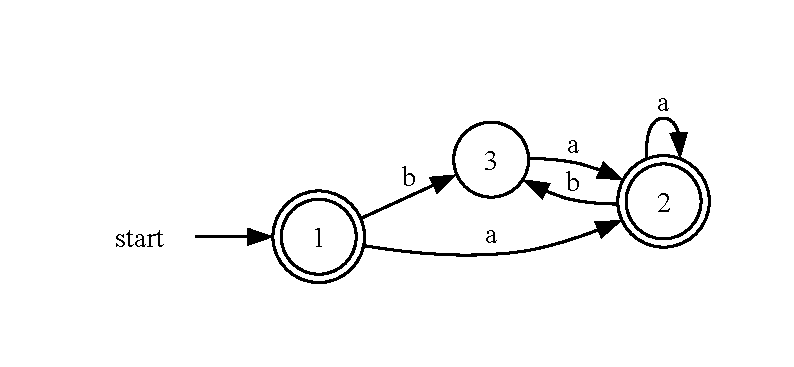
\includegraphics[width=\textwidth]{assets/dfa.pdf}
    \caption{dfa}
\end{figure}

\paragraph{2.} 请将其最小化

显然没有无效状态

首先将状态分为终态和非终态两个集合,\{3\},\{1,2\}

显然1,2不可分

得到最小化的DFA如下

\begin{figure}[H]
    \centering
    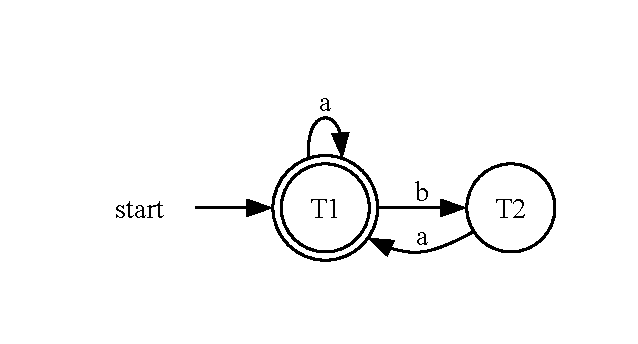
\includegraphics[width=\textwidth]{assets/mini-dfa.pdf}
\end{figure}

\section{符号表构造与运行时存储分析}

\paragraph{题干} 有如下程序段

\paragraph{1.} 说明符号表的内容和分程序索引表的作用

\begin{itemize}
    \item 符号表:是编译程序用来记录源程序中各种名字的特性信息,名字(程序名、过程名、函数名),特性信息(名字种类、类型、维数、参数个数、数值、目标地址等等)
    \item 分程序索引表:用于记录子符号表在主符号表的索引信息(帮助编译器快速定位到当前作用域的符号)
\end{itemize}

\paragraph{2.} 说明动态存储分配和静态存储分配的区别

\begin{itemize}
    \item 静态存储分配:在编译阶段由编译程序实现对存储空间的管理和为源程序中的变量分配存储的方法
    \item 动态存储分配:在目标程序运行阶段由目标程序实现对存储空间的组织与管理,和为源程序中的变量分配存储的方法
\end{itemize}

\paragraph{3.} 下图是递归计算斐波那契数列的C代码

\begin{lstlisting}
int f(int n){
    int t,s;
    if(n<2){
        return 1;
    }
    s=f(n-1);
    t=f(n-2);
    return s+t;
}
\end{lstlisting}

假设初始调用是f(5),调用f(5)时,运行栈的内容如下所示:

\begin{table}[H]
    \centering
    \begin{tabular}{|p{3cm}<{\centering}|p{2cm}<{\centering}|}
        \hline
               &      \\
        \hline
        s      &      \\
        \hline
        t      &      \\
        \hline
        n=5    &      \\
        \hline
        return &      \\
        \hline
        abp0   & abp1 \\
        \hline
    \end{tabular}
\end{table}

\paragraph{3.1} 请画出当第一个f(3)调用即将返回时运行栈的内容

\begin{table}[H]
    \centering
    \begin{tabular}{|p{3cm}<{\centering}|p{2cm}<{\centering}|}
        \hline
        s      &      \\
        \hline
        t      &      \\
        \hline
        n=3    &      \\
        \hline
        return &      \\
        \hline
        abp0   &      \\
        \hline
        abp1   &      \\
        \hline
        abp2   & abp3 \\
        \hline
        s      &      \\
        \hline
        t      &      \\
        \hline
        n=4    &      \\
        \hline
        return &      \\
        \hline
        abp1   &      \\
        \hline
        abp0   & abp2 \\
        \hline
        s      &      \\
        \hline
        t      &      \\
        \hline
        n=5    &      \\
        \hline
        return &      \\
        \hline
        abp0   & abp1 \\
        \hline
    \end{tabular}
\end{table}

\paragraph{3.2} 请画出第二个f(3)调用即将返回时运行栈的内容

\begin{table}[H]
    \centering
    \begin{tabular}{|p{3cm}<{\centering}|p{2cm}<{\centering}|}
        \hline
        s      &      \\
        \hline
        t      &      \\
        \hline
        n=3    &      \\
        \hline
        return &      \\
        \hline
        abp1   &      \\
        \hline
        abp0   & abp2 \\
        \hline
        s      &      \\
        \hline
        t      &      \\
        \hline
        n=5    &      \\
        \hline
        return &      \\
        \hline
        abp0   & abp1 \\
        \hline
    \end{tabular}
\end{table}

\section{LL(1)分析法}

\paragraph{题干} 有如下文法G[S]

\begin{equation}
    \begin{aligned}
        S & \rightarrow cAtSB|a     \\
        B & \rightarrow eA|\epsilon \\
        A & \rightarrow b
    \end{aligned}
\end{equation}

\paragraph{1.} 计算每个产生式右端符号串的FIRST集和每个非终结符的FOLLOW集(用\#代表输入结束)

\begin{table}[H]
    \centering
    \begin{tabular}{|p{3cm}<{\centering}|p{2cm}<{\centering}|}
        \hline
        \diagbox{符号串}{集合} & FIRST            \\
        \hline
        cAtSB|a           & \{c,a\}          \\
        \hline
        eA|$\epsilon$     & \{e,$\epsilon$\} \\
        \hline
        b                 & \{b\}            \\
        \hline
    \end{tabular}
\end{table}

\begin{table}[H]
    \centering
    \begin{tabular}{|p{4cm}<{\centering}|p{2cm}<{\centering}|}
        \hline
        \diagbox{非终结符}{集合} & FOLLOW     \\
        \hline
        S                  & \{e,t,\#\} \\
        \hline
        B                  & \{e,t,\#\} \\
        \hline
        A                  & \{e,t,\#\} \\
        \hline
    \end{tabular}
\end{table}

\paragraph{2.} 说明该文法是否为LL(1)文法,并给出依据

\begin{table}[H]
    \centering
    \begin{tabular}{|p{3cm}<{\centering}|p{2cm}<{\centering}|}
        \hline
        \diagbox{推导}{集合}        & SELECT     \\
        \hline
        $S\rightarrow cAtSB$    & \{c\}      \\
        \hline
        $S\rightarrow a$        & \{a\}      \\
        \hline
        $B\rightarrow eA$       & \{e\}      \\
        \hline
        $B\rightarrow \epsilon$ & \{e,t,\#\} \\
        \hline
        $A\rightarrow b$        & \{b\}      \\
        \hline
    \end{tabular}
\end{table}

各产生式推导分支的SELECT集有交集,因此不是LL(1)文法

\section{算符优先分析法}

\paragraph{题干} 有如下文法G[E]

\begin{equation}
    \begin{aligned}
        E & \rightarrow a|b|(A) \\
        A & \rightarrow EdA|E
    \end{aligned}
\end{equation}

\paragraph{1.} 求各非终结符的FIRSTVT和LASTVT集合

\begin{table}[H]
    \centering
    \begin{tabular}{|p{2cm}<{\centering}|p{1cm}<{\centering}|p{1cm}<{\centering}|p{1cm}<{\centering}|p{1cm}<{\centering}|p{1cm}<{\centering}|}
        \hline
        FIRSTVT & a & b & ( & ) & d \\
        \hline
        E       & 1 & 1 & 1 &   &   \\
        \hline
        A       & 1 & 1 & 1 &   & 1 \\
        \hline
    \end{tabular}
\end{table}

\begin{table}[H]
    \centering
    \begin{tabular}{|p{2cm}<{\centering}|p{1cm}<{\centering}|p{1cm}<{\centering}|p{1cm}<{\centering}|p{1cm}<{\centering}|p{1cm}<{\centering}|}
        \hline
        LASTVT & a & b & ( & ) & d \\
        \hline
        E      & 1 & 1 &   & 1 &   \\
        \hline
        A      & 1 & 1 &   & 1 & 1 \\
        \hline
    \end{tabular}
\end{table}

\paragraph{2.} 构造文法G的优先关系矩阵,并判断该文法是否是算符优先文法

\begin{table}[H]
    \centering
    \begin{tabular}{|p{2cm}<{\centering}|p{1cm}<{\centering}|p{1cm}<{\centering}|p{1cm}<{\centering}|p{1cm}<{\centering}|p{1cm}<{\centering}|}
        \hline
        优先关系 & a          & b          & (          & )         & d          \\
        \hline
        a    &            &            &            & $\gtrdot$ & $\gtrdot$  \\
        \hline
        b    &            &            &            & $\gtrdot$ & $\gtrdot$  \\
        \hline
        (    & $\lessdot$ & $\lessdot$ & $\lessdot$ & $\doteq$  & $\lessdot$ \\
        \hline
        )    &            &            &            & $\gtrdot$ & $\gtrdot$  \\
        \hline
        d    & $\lessdot$ & $\lessdot$ & $\lessdot$ & $\gtrdot$ & $\lessdot$ \\
        \hline
    \end{tabular}
\end{table}

该文法是算符优先文法,因为优先关系矩阵内没有重复项

\section{SLR分析法}

\paragraph{题干} 有如下文法G[S]

\begin{equation}
    \begin{aligned}
        S\rightarrow S0S0|S1S1|*
    \end{aligned}
\end{equation}

\paragraph{1.} 拓广文法,并求拓广后的文法后所有非终结符的FIRST集和FOLLOW集合

\begin{equation}
    \begin{aligned}
        S^{'} & \rightarrow S           \\
        S     & \rightarrow S0S0|S1S1|*
    \end{aligned}
\end{equation}

\begin{table}[H]
    \centering
    \begin{tabular}{|p{4cm}<{\centering}|p{2cm}<{\centering}|}
        \hline
        \diagbox{非终结符}{集合} & FIRST \\
        \hline
        $S^{'}$            & \{*\} \\
        \hline
        S                  & \{*\} \\
        \hline
    \end{tabular}
\end{table}

\begin{table}[H]
    \centering
    \begin{tabular}{|p{4cm}<{\centering}|p{2cm}<{\centering}|}
        \hline
        \diagbox{非终结符}{集合} & FOLLOW     \\
        \hline
        $S^{'}$            & \{0,1,\#\} \\
        \hline
        S                  & \{0,1,\#\} \\
        \hline
    \end{tabular}
\end{table}

\paragraph{2.} 求LR(0)项目集规范族,并分别给出能够识别活前缀S0S和S0S0的有效项目集

S0S

\begin{equation}
    \begin{aligned}
        S & \rightarrow S0S\cdot0 \\
        S & \rightarrow S\cdot0S0 \\
        S & \rightarrow S\cdot1S1
    \end{aligned}
\end{equation}

S0S0

\begin{equation}
    \begin{aligned}
        S & \rightarrow S0S0\cdot  \\
        S & \rightarrow S0\cdot S0 \\
        S & \rightarrow \cdot *    \\
        S & \rightarrow \cdot S0S0 \\
        S & \rightarrow \cdot S1S1
    \end{aligned}
\end{equation}

\section{代码优化}

\end{document}